\chapter{Technologien}\label{chap:technologies}
Eine den Anforderungen entsprechende Technologie zur Lösung einer Problemstellung auszuwählen ist eine notwendige, jedoch nicht hinreichende Bedingung für Erfolg. Aufgrund dessen sind die auf dem Markt verfügbaren Produkte sorgfältig gegeneinander abzuwägen. Dieses Kapitel beschreibt, welche Technologien für welchen Teil der Architektur in Frage kommen, stellt diese gegenüber und begründet die Entscheidung für die am besten geeignetste Alternative.

\section{Entwicklungsumgebung}
Die Entwicklung des \nameformat{\gls{crm}} findet zurzeit ausschließlich mit \nameformat{Microsoft Visual Studio} statt. Wie in Kapitel~\ref{chap:requirements} ausgeführt, gibt es die Core- und die Desktopkomponente, welche beide in \nameformat{C++} geschrieben sind, sowie eine auf den Core aufsetzende, in \nameformat{C\#} geschriebene, \nameformat{.NET}-Komponente zur Bereitstellung der Webfunktionalität. Eine künftige Entwicklung der Serverfunktionalität für die Weboberfläche kann auf der \nameformat{.NET}-Komponente aufsetzen bzw.\ diese erweitern. Dieser Entwicklungsprozess wird nicht verändert und auch nicht weiter thematisiert werden, da die neu zu entwickelnde UI-Schicht eine unabhängige Codebasis besitzt und sich auch konzeptionell von den bisherigen Schichten unterscheidet. Bei der Auswahl der neuen Technologien ist es daher nicht unbedingt notwendig, sich an bestehenden Abläufen zu orientieren. 

Das in Kapitel~\ref{chap:requirements} beschriebene Tool zum Einlesen und Konvertieren der bisherigen UI-Repräsentation wurde wegen der vorhandenen, internen Infrastruktur ebenfalls \nameformat{Visual Studio} verwendet. Als Sprache für die Entwicklung wurde \nameformat{C\#} gewählt, nicht zuletzt weil diese einen besonders unkomplizierten Zugriff auf das Dateisystem und speziell auf XML-Dateien, das Format der momentanen Repräsentation, erlaubt. 

Für die neu entstehenden Webtechnologien kann jeder beliebige Texteditor benutzt werden, da keine speziellen Funktionen einer IDE oder eines Editors notwendig sind. Der in den nachfolgenden Kapiteln entwickelte Code wurde aufgrund der guten Autovervollständigung, der Integration mit Versionsverwaltungstools und der einfachen Erweiterbarkeit, mit \nameformat{Visual Studio Code} von \nameformat{Microsoft} erstellt. Wichtiger als der Editor ist die Sprache, für welche er benutzt wird. Im Bereich der Webentwicklung hat sich \nameformat{JavaScript} ohne Konkurrenz durchgesetzt und ist daher auch die einzige Sprache, die von allen Browsern unterstützt wird. Dies spiegelt sich auch in der Auswahl der Frontend-Frameworks wider, welche ausnahmslos entweder direkt oder indirekt in \nameformat{JavaScript} geschrieben sind.   

\section{Frontend-Frameworks}
Frameworks und Bibliotheken, die versuchen, Entwicklern das Erstellen von UIs zu erleichtern, gibt es schon seit geraumer Zeit und in einer sehr großen Anzahl. Etablierte Projekte wie \nameformat{jQuery-UI} (Mobile), \nameformat{Bootstrap} und neuere Projekte (\nameformat{Materialize}, \nameformat{Semantic-UI}, \nameformat{Pure} etc.) setzen auf die Gestaltung von fertigen Komponenten, die per \nameformat{CSS}-Klasse in eine vorhandene Webseite integriert werden können. Durch diesen Fokus auf Styling mit \nameformat{CSS} sind diese Projekte meist sehr klein und können schnell integriert werden. Sie eignen sich damit für Prototypen, welche rapiden Änderungen unterliegen, jedoch nicht für die vollständige Erstellung kompletter Webseiten. Sie können vielmehr im Zusammenspiel mit den zuvor angesprochenen \nameformat{JavaScript}-Projekten benutzt werden.

Im Bereich moderner \nameformat{JavaScript}-Lösungen sind vor allem komponentenbasierte Frameworks, welchen eine virtuellen DOM\footnote{Virtuelle und meist vereinfachte Repräsentation der UI im Speicher, wird Framework-intern mit dem tatsächlichen DOM der Seite synchronisiert} zugrunde liegt, stark verbreitet. Aufgrund der zeitlichen Limitierung dieser Arbeit können nicht sämtliche Alternativen gegeneinander abgewogen werden. Es werden daher nur die drei größten Mitstreiter \nameformat{Vue}, \nameformat{React} und \nameformat{Angular} \parencite[vgl.][]{greif_benitte_rambeau_2018} miteinander verglichen. Weitere Möglichkeiten für spätere Analysen sind \nameformat{Polymer}, \nameformat{Ember}, \nameformat{Knockout}, \nameformat{Riot}, und Weitere.

In den folgenden Abschnitten werden verschiedene, bei der Entwickler einer Webapplikation wichtige Gesichtspunkte und deren Umsetzung in den entsprechenden Frameworks beschrieben. Dies dient dem Überblick über die für die Entscheidung relevanten Betrachtungen und zur besseren Nachvollziehbarkeit des im Anschluss gezogenen Fazits.

\subsection{Generelle Aspekte}
Die Entwickler von \nameformat{Vue} legen besonderen Wert auf die Entwicklung einer möglichst kleinen und dennoch performanten Laufzeit-Umgebung. Das Ziel einer kurzen Einarbeitungszeit sowie einer intuitiven Handhabung wird durch eine sehr gute Dokumentation und ein hervorragendes \gls{cli}-Tool zum Erstellen neuer Projekte erreicht. Abhängigkeiten zwischen Daten und UI ermittelt \nameformat{Vue} selbstständig, es werden daher immer nur Elemente aktualisiert, wenn sich auch deren anzuzeigende Daten geändert haben. Das Erstellen von nativen Apps ist bei \nameformat{Vue} nur mit Software von Drittherstellern möglich. Um diesem Nachteil entgegenzuwirken und den Prozess der Weiterentwicklung zu optimieren, arbeiten die Entwickler eng mit den Drittherstellern zusammen. Das Verwenden von \nameformat{JavaScript}-Templates (JSX) und \nameformat{TypeScript} ist mit vorheriger Konfiguration ebenfalls möglich. \nameformat{Vue} hat ein vergleichsweise kleines Ökosystem, kann dafür aber das stärkste Wachstum aller Frameworks verzeichnen \parencite[vgl.][]{npmjs_2018}.

\nameformat{React} diktiert im Vergleich zu \nameformat{Vue} noch weniger Vorgaben an die Entwickler, sämtliche typischen Problemstellungen werden durch Bibliotheken gelöst. Der Hintergrund hierfür ist das umfassende Ökosystem sowie eine breite Auswahl an entsprechenden Bibliotheken. Native Apps (\nameformat{Android}, \nameformat{iOS}) können mit dem vom gleichen Team entwickelten \nameformat{React-Native} erstellt werden, ohne dass sie dafür weitere Software benötigen. Durch die Konzentration auf wesentliche Features und Verbesserungen sowie eine stabile API stellt das \nameformat{React}-Team sicher, dass Upgrades auf neue Versionen gar keine bis wenige Änderungen am bestehenden Code verlangen. Auch \nameformat{TypeScript}-Integration und damit verbundenes Tooling (Linter, Typ-Prüfung, Autovervollständigung) sind problemlos möglich.

Im Fall von \nameformat{Angular} werden zur Erfüllung aller typischen Anforderungen die bei der Entwicklung anfallen, bereits Tools und Konzepte mit ausgeliefert. Dadurch ist \nameformat{Angular} an sich sehr viel mächtiger als \nameformat{Vue} und \nameformat{React}. Die Wahrscheinlichkeit dafür, dass abgesehen von \nameformat{Angular} noch weitere große Bibliotheken benötigt werden, ist gering. Die Nutzung dieser mitgelieferten Möglichkeiten erfordert jedoch auch, dass ausreichend Kenntnisse über sie vorhanden sind. Diese Notwendigkeit, viele Teilaspekte des Frameworks lernen zu müssen, macht den Einstieg in \nameformat{Angular} daher relativ mühsam und zeitintensiv. Die Dokumentation ist zwar sehr umfangreich, teilweise aber auch unübersichtlich. Das Ökosystem von \nameformat{Angular} ist noch größer als das von \nameformat{Vue}, es hat jedoch auch negatives Wachstum zu verzeichnen \parencite[vgl.][]{npmjs_2018}.

\subsection{Aufbau von Apps (mit Beispielkomponente)}
Zur Veranschaulichung der Benutzung der Frameworks wurde eine ausgewählte Beispielkomponente mit jedem der drei Frameworks umgesetzt. In Abbildung~\ref{fig:example_component} ist die fertige Komponente dargestellt. Bei einem Klick in das Edit-Feld ändert sich die Farbe des Rahmens, um die Fokussierung zu signalisieren. Wird der Eintrag verändert, kann diese Änderung mit Escape verworfen oder mit Enter übernommen werden. Der Text darunter gibt immer den momentan gespeicherten Wert wieder. Die Komponente wurde in Online-Editoren erstellt, welche bereits eine fertige Umgebung mit dem jeweiligen Framework bieten. Auf die Benutzung weiterer Bibliotheken wurde hier explizit verzichtet.

\begin{figure}
    \centering
    \captionsetup{justification=centering}
    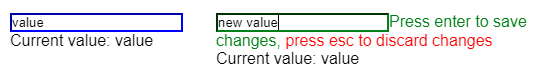
\includegraphics[width=\textwidth]{figures/example_component.png}
        \caption{Beispielkomponente für die Umsetzung mit allen Frameworks}\label{fig:example_component}
\end{figure}

Die \nameformat{Vue}-Komponente wird vollständig als Instanz einer \nameformat{Vue}-Klasse angelegt, der Daten und Methoden übergeben werden müssen. Im HTML-Template werden die \nameformat{Vue}-eigenen Attribute ersichtlich. Eine Implementierung ist in Auflistung~\ref{lst:vue_example} dargestellt.

\lstinputlisting[language={JavaScript}, label={lst:vue_example},caption={Umsetzung der Beispielkomponente mit \nameformat{Vue}}]{code/chapter_003_vue_example.js}

Eine \nameformat{React}-Komponente kann entweder als herkömmliche Klasse, dargestellt in Auflistung~\ref{lst:react_example}, oder nur als Funktion, welche die darzustellenden UI-Elemente als Rückgabewert enthält, angegeben werden. Eine Umsetzung der zweiten Umsetzung ist im Anfang~\ref{lst:appendix_react_hooks_example} dargestellt.

\lstinputlisting[language={JavaScript}, label={lst:react_example},caption={Umsetzung der Beispielkomponente mit \nameformat{React}}]{code/chapter_003_react_example.js}

Bei \nameformat{Angular} besteht eine Komponente wie bei \nameformat{React} aus einer herkömmlichen Klasse. Diese wird jedoch mit einer speziellen Annotation mit Informationen über das Aussehen und die Platzierung der Komponente versehen.

\lstinputlisting[language={JavaScript}, label={lst:angular_example},caption={Umsetzung der Beispielkomponente mit \nameformat{Angular}}]{code/chapter_003_angular_example.js}

\subsection{Vergleich der Zustands-Verwaltung}
Jede Applikation muss früher oder später Daten speichern, also einen gewissen Zustand bewahren, um Nutzern mehr als nur die simpelsten Funktionalitäten anbieten zu können. Wie das Speichern dieser Daten mit den drei Frameworks typischerweise umgesetzt ist, wird in diesem Abschnitt beschrieben.

Der Standard bei \nameformat{Vue} ist, dass jede Komponente ihr eigenes Zustands-Objekt besitzt. Zusätzlich dazu kann noch auf das Zustands-Objekt der \nameformat{Vue}-Instanz, in der sich die Komponente befindet, zugegriffen werden. Dieses kann entweder direkt verändert, oder per Store-Pattern\footnote{Geteilter Zustand wird zentral verwaltet, Änderungen am Zustand nur intern möglich} verwaltet werden. \nameformat{Vuex} ist eine direkt von \nameformat{Vue} entwickelte Bibliothek, welche das genannte Store-Pattern umsetzt.

\nameformat{React} unterstützt nur einen unidirektionalen Datenfluss mit sogenannten \enquote{Props}\footnote{Unveränderbare Übergabeparameter}, welche den Komponenten von ihren Elternkomponenten mitgegeben werden. Jede Komponente hat ihren eigenen Zustand, der per \enquote{Props} an Kinder weitergegeben, aber nicht direkt verändert, werden kann. Es gibt einige bekannte Bibliotheken, welche die Verwaltung von Zustand auf andere Arten lösen. \nameformat{Redux} setzt beispielsweise das funktionale Flux-Pattern um. Dabei werden Änderungen per Aktions-Event ausgelöst, die Events von sogenannten Reducern ausgewertet und der Zustand von diesen entsprechend verändert. Der neue Zustand wird den entsprechenden UI-Elementen wieder unveränderbar (immutable) übergeben. \nameformat{MobX} und \nameformat{react-easy-state} setzen das bei \nameformat{Vue} erwähnte Store-Pattern in \nameformat{React} um.

Bei \nameformat{Angular} wird der Zustand direkt in den Klasseninstanzen der Komponenten gespeichert und kann durch herkömmliche Konzepte der objektorientierten Programmierung weitergegeben und verändert werden. Zusätzlich existiert auch \nameformat{NGXS}, welches auf demselben Prinzip wie \nameformat{Redux} beruht, aufgrund der Nutzung moderner \nameformat{TypeScript}-Features von \nameformat{Angular} aber ohne weitere Konfiguration einfacher zu benutzen ist.

\subsection{Vergleich von Routing-Konzepte}
Unter Routing versteht man das Konzept, dass bei Navigation zu Subdomänen einer Webseite automatisiert die dafür vorgesehene Komponente dargestellt wird.

Routing ist bei \nameformat{Vue} direkt integriert. Routen werden in \nameformat{JavaScript} mit Komponenten verknüpft und bei Aufruf dieser Route wird die verknüpfte Komponente anstatt eines zuvor im DOM platzierten Platzhalters gerendert.

\nameformat{React} besitzt keine integrierten Routing-Mechanismen, es gibt aber mehrere Alternativen als Bibliotheken. Bei \nameformat{Aviator} werden Routen als geschachteltes Objekt übergeben, bei dem jedes Element eine Route und eine Zielfunktion enthält. Die Zielfunktion wird aufgerufen, wenn zur entsprechenden Route navigiert wird. Sie muss des Weiteren Informationen darüber enthalten, wie und an welche Stelle im DOM (etwa über Dokument-Selektoren) die entsprechende Komponente gerendert werden soll. Die Nutzung von JSX ist dabei nicht mehr möglich. Bei \nameformat{react-router} hingegen werden die Routen deklarativ in den JSX-Templates hinterlegt. Sie enthalten als Property die Route, für die sie gerendert werden sollen, sowie die eigentlich anzuzeigende Komponente.

Analog zu \nameformat{Vue} ist bei \nameformat{Angular} auch eine Lösung direkt integriert welche nach demselben Prinzip funktioniert.

\subsection{Vergleich der Testintegration}
\nameformat{Vue} enthält Test-Tools mit denen Komponenten in Variablen gerendert werden können. Diese gespeicherten Komponenten sind herkömmliche \nameformat{JavaScript}-Objekte und können dann mit weiteren (externen) Tools auf bestimmte Zustände und Eigenschaften geprüft werden. Das Testen von \nameformat{React}-Komponenten funktioniert analog zu \nameformat{Vue}.

Sämtliche zum Testen benötigten Tools sind bei \nameformat{Angular} bereits enthalten und sehr ausführlich dokumentiert. Wenn nur bestimmte Teilaspekte einer Anwendung, wie etwa die UI-Komponenten, getestet werden sollen, ist der Aufwand dies einzurichten aufgrund der Notwendigkeit, sich mit dem gesamten Test-Konzept auseinandersetzen zu müssen, höher als bei \nameformat{Vue} und \nameformat{React}.

\subsection{Vergleich der \acrlong{ssr}-Möglichkeiten}
Bei der Benutzung von \gls{ssr} werden die Seiten nicht auf dem Clientrechner, sondern bereits vor dem Senden auf dem Server gerendert. Es besteht bei allen Frameworks auch die Möglichkeit nur wenige Seiten \enquote{vor-gerendert} auf dem Server abzuspeichern, anstatt sie dynamisch bei entsprechenden Anfragen zu generieren. Hierfür kann das \nameformat{Node.js} Tool \nameformat{Prerender.io} benutzt werden.

\nameformat{Vue} liefert einen dafür vorgesehenen Renderer (\nameformat{vue-server-renderer}), der Markup als Text generiert. Dieser Markup-Text kann beim initialen Laden der Seite ausgeliefert werden (erfordert einen \nameformat{Node.js} Server).

Auch \nameformat{React} liefert einen dafür vorgesehenen Renderer (\nameformat{ReactDOMServer}), der Markup als Text generiert. Dieser kann analog zu \nameformat{Vue} ausgeliefert und auf Clientseite mit \enquote{ReactDom.hydrate()} mit Inhalten gefüllt werden (erfordert einen \nameformat{Node.js} Server).
    
Bei \nameformat{Angular} werden für \gls{ssr} zusätzliche Abhängigkeiten, Änderungen an der Konfiguration, ein zusätzliches Build / Bundle Target und ein zusätzliches Modul mit separater Konfiguration, das auf dem Server läuft und dafür zuständig ist, das neue \nameformat{JavaScript}-Bundle auszuliefern, benötigt.

\subsection{Fazit}
Alle betrachteten Alternativen sind geeignete Optionen zur Umsetzung der zuvor beschriebenen Anforderungen. Bezüglich der Funktionalität bestehen folglich keine Unterschiede, es kommt daher vielmehr darauf an, welches Projekt einem Entwickler (-team) am meisten zusagt bzw.\ mit welchem er (es) am besten arbeiten kann.
Die Einarbeitung in \nameformat{Angular} kann Schwierigkeiten bereiten, da dort eine Vielzahl an Technologien für verschiedene Zwecke mitgeliefert werden, welche für die Benutzung erlernt werden müssen. \nameformat{React} besitzt mit Abstand die größte Community, es kann somit davon ausgegangen werden, dass die Weiterentwicklung, zahlreiche aufsetzende Bibliotheken und Ressourcen im Netz garantiert sind. Ein weiterer Vorteil, die Benutzung von \nameformat{TypeScript} vorausgesetzt, ist die IDE-Unterstützung beim Schreiben der Komponenten-Templates. Im Vergleich zu \nameformat{Vue} wird bei \nameformat{React} hier ausschließlich \nameformat{JavaScript} genutzt, was es erlaubt, optional \nameformat{TypeScript} einzusetzen und dessen Typisierung zu nutzen, um Autovervollständigung oder ähnliche Hilfen anzubieten. \nameformat{Vue} hingegen schreibt \nameformat{JavaScript}-Funktionsaufrufe in Strings und nutzt eigene, für nicht \nameformat{Vue}-Entwickler unbekannte, \nameformat{HTML}-Attribute für Schleifen und Verzweigungen. Da es sich dabei um \nameformat{Vue}-Sonderfälle handelt, kann die IDE oft nicht helfen. Es liegt folglich am Entwickler, das entsprechende Wissen aufzubauen und keine Fehler zu machen.

Nach Abwägung der diskutierten Punkte fiel die Entscheidung für den Prototypen vorerst auf die Nutzung von \nameformat{React}. Aufgrund der Tatsache, dass die Technologien nach dem Transpilierungsvorgang alle kompatibel sind (sie werden alle in herkömmliches \nameformat{HTML}, \nameformat{CSS} und \nameformat{JavaScript} übersetzt), kann dieser Code später jedoch auch mit \nameformat{Vue} zusammen genutzt oder allmählich durch alternative Komponenten ersetzt werden.

\section{TypeScript}
Bei \nameformat{JavaScript} handelt es sich um eine dynamisch typisierte Sprache, das heißt, dass sich Typen von Variablen zur Laufzeit ändern können und vor der Nutzung einer Variablen entsprechend überprüft werden müssen. Dies ist ein Vorteil, wenn innerhalb kurzer Zeit kleinere Skripte geschrieben werden, bei denen aufgrund ihrer überschaubaren Größe entsprechende Überprüfungen trivial sind, oder im Skript enthaltene Fehler vernachlässigbar sind. Für die Entwicklung von größeren Projekten ist diese Eigenschaft jedoch ein gravierender Nachteil, da Typen von Variablen im Code durch Entfernung von Deklaration und Nutzung nicht ersichtlich sind. Daraus resultierende Fehler treten bei der Benutzung immer erst zur Laufzeit der betroffenen Zeilen auf, oder sind sogar gar nicht als Fehler erkennbar und liefern lediglich ein falsches (aber nicht unbedingt als falsch erkennbares) Ergebnis.  

Um dieser Art von subtilen Bugs vorzubeugen, bietet \nameformat{Microsoft} seit 2012 \nameformat{TypeScript} an. Es handelt sich dabei um eine typisierte open-source Sprache, welche als syntaktische Obermenge von \nameformat{JavaScript} (gewöhnlicher \nameformat{JavaScript}-Code ist also ebenso gültiger \nameformat{TypeScript}-Code) beschrieben werden kann. Sie wird zu gewöhnlichem \nameformat{JavaScript} transpiliert und besitzt somit trotz ihrer Vorteile keinen Kompatibilitätsnachteil. Da die Syntax auf \nameformat{JavaScript} basiert, ist das Erlernen dieser für \nameformat{JavaScript}-Entwickler trivial. Durch Verwendung typisierter Daten wird die fehlerhafte Nutzungen der Variablen bereits bei der Entwicklung --- eine entsprechende Integration des Editors vorausgesetzt --- oder spätestens beim Transpilieren bemerkt und dem Entwickler als solche angezeigt. Ebenso erlaubt eine Editorintegration die Bereitstellung einer Codevervollständigung, was Entwicklern häufig die Konsultation der Dokumentation erspart und damit zu einem effektiveren Entwicklungsprozess beiträgt.

Der einzige Nachteil von \nameformat{TypeScript} ist, dass ein zusätzlicher Schritt zum Übersetzen in \nameformat{JavaScript}-Code notwendig ist. 
Die Mehrheit der Projekte im Webbereich setzt jedoch ohnehin vergleichbare Tooling-Schritte voraus, in welche das Kompilieren integrierbar ist, sodass die genannte Einschränkung weniger stark ins Gewicht fällt. Dieser Nachteil kann aber auch positiv ausgelegt werden: durch den Übersetzungsschritt ist es möglich, bereits Features und Standards zu benutzen, welche noch nicht von allen Browsern unterstützt werden. Bei der Übersetzung werden diese in semantisch identischen Code umgewandelt, der unter Einhaltung von älteren Standards gültig ist, aber für den Entwickler schwieriger zu schreiben wäre. 

Aufgrund dieser Argumentation soll zur Unterstützung der Entwickler und Vorbeugung von Fehlern bei der Entwicklung der \nameformat{React}-Seite ausschließlich \nameformat{TypeScript} benutzt werden. 

\section{API-Anbindung}
Für die Anbindung der API kommen zwei Ansätze in Frage: \nameformat{REST} und \nameformat{GraphQL}\@. Bei \nameformat{REST} handelt es sich um einen Architekturstil, bei dem Ressourcen über URI-Endpunkte angesprochen und abgerufen werden. \nameformat{GraphQL} hingegen ist eine von \nameformat{Facebook} entwickelte Query-Sprache zur Abfrage von vorhandenen Daten. In den folgenden Abschnitten werden speziell die für dieses Projekt relevanten Vor- und Nachteile beider Ansätze angesprochen.

\subsection{Abwägung von REST für die API-Anbindung}
\nameformat{REST}-APIs sind heutzutage die Norm, diese Architektur allerdings korrekt umzusetzen, ist jedoch mit viel Arbeit und gewissen Nachteilen verbunden. Dies könnte einer der Gründe dafür sein, dass ein großer Teil der angesprochenen \nameformat{REST}-APIs nur \enquote{REST-like} sind. Als \enquote{REST-like} werden die Implementationen bezeichnet, welche das sogenannte HATEOAS~\footnote{Hypermedia as the Engine of Application State}-Konzept nicht umsetzen. Das Konzept beschreibt, wie ein Client durch die API navigieren soll --- alle validen Übergänge vom momentanen Zustand in den nächsten sind bereits in der Antwort einer Anfrage in Form von Links und Metadaten verfügbar. Ein Konsument muss damit nicht mehr wissen, welche Anfragen zu welchem Zeitpunkt gültig sind und kann immer genau die Aktionen anbieten, die auch von der API angeboten werden. Eine Versionierung der API (und damit stärkere Kopplung zwischen Clients und Server) entfällt ebenfalls, neue Features können als weitere Aktion-Links auftauchen und alte, bald nicht mehr verfügbare Features können neben einem Link mit der Information versehen werden, dass sie nicht weiter genutzt werden sollten. Trotz verschiedener Standards, die beim Erstellen der Struktur der Daten helfen, ist es aufgrund des Mehraufwands bei jedem Endpoint dennoch mühsam, eine \nameformat{REST}-API mit HATEOAS korrekt zu implementieren. Zusätzlich dazu, und dieser Nachteil wird im Gegenzug zu der gerade beschriebenen Flexibilität absichtlich in Kauf genommen, können solche APIs nur navigiert werden, indem vielen Links gefolgt und damit viele Netzwerkanfragen vorgenommen werden. 
Die Alternative, \nameformat{REST}-APIs ohne HATEOAS zu erstellen, ist zwar für die Entwickler einfacher, das Konsumieren der API wird dadurch aber deutlich erschwert. Eine Anbindung ist nur durch eine ständige Konsultation der Dokumentation (welche in entsprechender Qualität vorhanden sein muss) möglich. Bei Änderungen an der API müssen auch die Clients angepasst werden, da es keine Möglichkeit gibt sie über diese Änderungen dynamisch zu informieren.
Zur Vereinfachung der Erstellung konzeptionell korrekter \nameformat{REST}-APIs gibt es den \nameformat{OData}-Standard, der Entwicklern unter anderem die Definition und die Erstellung von Metadaten abnimmt, sodass diese sich auf die eigentliche Programmlogik konzentrieren können.

Caching ist bei \nameformat{REST} einfacher möglich als bei \nameformat{GraphQL}: hier kann jedes Endpoint-Daten-Paar als ein Eintrag im Cache angesehen werden. Sind entsprechende Cache-Header in den HTTP-Nachrichten gesetzt, werden die Daten vom Browser (und eventuell vorhandenen Cache-Proxies) automatisch verwaltet. Dies funktioniert, weil Anfragen einer Ressource bei \nameformat{REST} immer alle Daten erhalten, die es zu dieser Ressource gibt. Um nicht immer alle Daten übertragen zu müssen, besitzen viele \nameformat{REST}-APIs Parameter, mit denen eine Anfrage einschränkt werden kann. Je feiner diese Einschränkungen sein können, desto weniger überflüssige Daten müssen übertragen werden. Gleichzeitig greift damit aber auch der HTTP-Cache immer seltener, weil dauerhaft verschiedene Endpoint-Daten-Paare angefragt werden.

\subsection{Abwägung von GraphQL für die API-Anbindung}\label{subsec:graphql}
Einer der Hauptgründe für die Entwicklung von \nameformat{GraphQL} ist die höhere Netzwerklast bei \nameformat{REST}-APIs, die insbesondere bei mobilen Clients sehr negativ auffallen kann. Ein Hauptaugenmerk der Technologie liegt daher auf der größtmöglichen Sparsamkeit bzgl.\ der Größe übertragener Daten.
\nameformat{GraphQL} ist laut \nameformat{npm} die im Webbereich mit am meisten wachsende Technologie überhaupt (\enquote{hyper-growth} \parencite*[vgl.][]{npmjs_2018}). Als Folge dessen wird es in Zukunft wahrscheinlich in vielen Projekten benutzt werden, der Aufbau von entsprechendem Know-How ist daher essentiell.
Eine Abfrage bei \nameformat{GraphQL} hat den gleichen Aufbau wie ein JSON-Dokument, mit der Besonderheit, dass anstatt Schlüssel-Werte-Paaren nur Schlüssel bzw.\ die Namen von Ressourcen angegeben werden. Eine Antwort hat immer den gleichen Aufbau wie eine Anfrage, die Schlüssel bzw. Ressourcennamen werden dabei, wie in Listing~\ref{lst:graphql_example_query} zu sehen, mit den ausgelesenen Daten ergänzt. Durch die Nutzung von Typen für diese Abfragen kann garantiert werden, dass eine von den Tools akzeptierte Anfrage auf jeden Fall ein Ergebnis vom Server liefern wird. Die Abfragen müssen dabei nicht alle Felder einer Ressource enthalten, es können immer genau die Daten abgefragt werden, die in einer spezifischen Situation gerade benötigt werden. Ebenfalls können mehrere unabhängige Anfragen zu einer großen Anfrage zusammengefasst und mit nur einer Netzwerkanfrage verarbeitet werden.
Das typisierte Schema erlaubt weiterhin, Konsumenten jederzeit Informationen über sich selbst (Metadaten), etwa den Typ eines Feldes oder weitere mögliche Felder zur Abfrage, zur Verfügung zu stellen. Vorausgesetzt ein Client kennt einen der Einsprungspunkte eines Graphen, kann er mit diesen Metainformationen alle weiteren Informationen programmatisch auslesen. 

\lstinputlisting[language={JavaScript}, label={lst:graphql_example_query},caption={Beispielquery aus der \nameformat{GraphQL} Dokumentation \parencite{graphql_doc_example_query}}]{code/chapter_003_graphql_example_query.js}

Um Entwickler zu unterstützen, existiert ein visueller Query-Editor \nameformat{GraphiQL} mit Autovervollständigung sowie aus dem Schema generierter Dokumentation. Mithilfe dieses Editors kann einerseits sehr leicht in der API navigiert und andererseits können direkt code-seitig benutzbare Abfragen generiert werden.
Viele moderne Webseiten basieren nicht mehr nur auf der Annahme, dass irgendwann Daten vom Server abgefragt werden, sondern auch darauf, dass serverseitige Events / Änderungen das Laden oder Anzeigen von Daten auslösen können. \nameformat{GraphQL} spezifiziert für diese Anforderung ein Abonnement-System: ein Client registriert sich beim Server für alle Daten, über deren Änderung er umgehend informiert werden möchte und gibt an, welche Abfrage dafür ausgeführt werden soll. Bei einer Änderung wird diese Abfrage dann ausgeführt und die Daten über eine Websocket-Verbindung sofort an den Client übertragen.

Um all diese Eigenschaften zu ermöglichen, ist es jedoch notwendig, dass sowohl der Client als auch der Server mit demselben \nameformat{GraphQL}-Schema arbeiten und damit aneinander gekoppelt sind.
Ein weiterer Nachteil ist es, dass aufgrund der Nutzung von \nameformat{GraphQL} (nur HTTP-POST und identischer Endpoint) Caching nicht auf HTTP-Ebene geschehen kann und damit die Verantwortung für gute Cache-Strategien hauptsächlich beim Client liegen.

Zwei bekannte Bibliotheken, welche die \nameformat{GraphQL}-Spezifikation in \nameformat{JavaScript} umsetzen und für die Erstellung der Webseite genutzt werden können, sind \nameformat{Apollo} und \nameformat{Relay}. Sie erleichtern das Erstellen von Abfragen (\enquote{Queries}), Caching und Debuggen bei der Nutzung von \nameformat{GraphQL}\@. \nameformat{Relay} wurde ebenfalls von \nameformat{Facebook} entwickelt, dennoch hat \nameformat{Apollo} eine sehr viel größere Community. Für die Umsetzung im Backend (.NET) existieren ebenfalls Implementierungen, die am meisten genutzte davon ist \nameformat{graphql-dotnet}.

\subsection{Fazit}
\nameformat{REST} und \nameformat{GraphQL} können beide zur Erfüllung desselben Zwecks genutzt werden, sie konkurrieren jedoch nicht direkt miteinander. Eine API kann ebenso beide Ansätze entweder ergänzend oder parallel anbieten. Bestehende \nameformat{REST}-APIs können von \nameformat{GraphQL} auf einfache Art und Weise umhüllt und zusammengefasst werden. So können sie auf beide Arten angesprochen werden. \nameformat{REST} ist allerdings flexibler als \nameformat{GraphQL}\@. Um diese Flexibilität vernünftig zu nutzen und damit eine API zu schreiben, welche viele Jahre genutzt und skaliert werden kann, ist jedoch viel Erfahrung und Aufwand unverzichtbar. \nameformat{GraphQL} benötigt sowohl eine Server- als auch eine Clientkomponente und hat damit mehr Abhängigkeiten als dies bei \nameformat{REST} der Fall ist, im Gegenzug ist es dadurch aber möglich, effiziente und typsichere Anfragen zu erstellen. Ebenso wird mit dem mitgelieferten \nameformat{GraphiQL}-Tool ein Abfrage-Editor mit Autovervollständigung und Fehlerbeschreibungen bereitgestellt, der den Nutzern die Erkundung einer API und deren Möglichkeiten erleichtert, sowie für alle Bestandteile direkt eine Dokumentation generiert. \nameformat{GraphQL} scheint daher als die sinnvollere Wahl für Firmen oder Personen, die noch nicht viel Erfahrung bei der Erstellung von APIs sammeln konnten. Ein weiterer wichtiger Vorteil von \nameformat{GraphQL} ist es, dass durch die typisierten Abfragen eine automatische Generierung von Mocking-Daten möglich ist. Mithilfe solcher Mocking-Daten kann das Entwicklerteam den API Client im Frontend entwickeln und testen, bevor das Backend mit den Echtdaten zur Verfügung steht.

Wegen der einfacheren Nutzung von \nameformat{GraphQL} und der besseren Unterstützung von Entwicklern durch Typisierung und mitgelieferten Tools wird im Prototyp diese Technologie verwendet.
